\chapter{Introducción específica} % Main chapter title

\label{Chapter2}

%----------------------------------------------------------------------------------------
%	SECTION 1
%----------------------------------------------------------------------------------------
Este capítulo explica las tecnologías aplicadas en el desarrollo de la pantalla gigante \textit{full color}. Se presentan los requerimientos identificados al iniciar el trabajo para cumplir con los objetivos.
\section{Matriz de LEDs}
La matriz de LEDs es un conjunto o arreglo de LEDs  bidimensional donde los cátodos se unen en filas y los ánodos se unen en columnas. Existen numerosos métodos para controlar las matrices de LEDs. Para desarrollar este proyecto se seleccionó el método de multiplexación debido a su bajo uso de recursos en comparación a controlar los LEDs de manera individual \citep{CONCEPTOMATRIZ}.

\subsection{LED SMD CLX6F}
Los principales productores de LEDs son CREE, EPISTAR, NICHIA, SEOUL SEMICONDUCTOR, Toyoda Gosei y Agilent.
El LED que fue elegido para la construcción de la pantalla fue el CLX6F que forma parte del catálogo de productos de la empresa CREE. Se logró contactar con una empresa en Shenzhen que usaba el \textit{chip} de CREE pero agregaba un encapsulado propio, lo que abarató el precio. El producto seleccionado es un LED tricolor diseñado para ser usado en pantallas exteriores de vídeo, sus características principales son:



\begin{itemize}
\item Resistencia al agua IPX8.
\item Luminosidad del rojo 560 mcd a 1120 mcd.
\item Luminosidad del verde 900 mcd a 1800 mcd.
\item Luminosidad del azul 140 mcd a 355 mcd.
\item El encapsulado del LED contiene inhibidores de UV lo cual minimiza el efecto a largo plazo de los rayos solares.
\end{itemize}

Las características eléctricas máximas se muestran en la tabla \ref{tab:MAXLEDCLX6F}.

\pagebreak


\subsection{Driver de LED MBI5051}
El driver que se eligió para habilitar las columnas de LEDs fue el MBI5051. Este es un producto de la empresa MACROBLOCK. En diseños anteriores se usaron productos similares de esta empresa. EL MBI5051 fue diseñado para ser usado en pantallas exteriores de vídeo. Las características del driver se muestran en la tabla \ref{tab:driverled}.
 
\begin{table}[h]
\centering
\caption[Características eléctricas máximas LED CLX6F]{Características eléctricas máximas LED SMD CLX6F \protect\footnotemark.}
\begin{tabular}{l c c c c}
\toprule
\textbf{Especificaciones}& \textbf{R} & \textbf{G} & \textbf{B}\\
\midrule 


Corriente directa &50 mA &35 mA &35 mA\\
Corriente directa pico &200 mA &100 mA &100 mA \\
Voltaje inverso &5 V &5 V &5 V\\
Temperatura de operación &-40 \si{\degree}C a 100 \si{\degree}C  &-40 \si{\degree}C a 100 \si{\degree}C  &-40 \si{\degree}C a 100 \si{\degree}C\\


\bottomrule
\hline
\end{tabular}
\label{tab:MAXLEDCLX6F}
\end{table}

\footnotetext{Referencia tomada de \url{https://cree-led.com/media/documents/ds-CLX6F-FKC-1352.pdf}}

\begin{table}[h]
\centering
\caption[Características MBI5051]{Características del driver MBI5051 \protect\footnotemark.}
\begin{tabular}{l c c}
\toprule
\textbf{Especificaciones}& \textbf{Detalles}\\
\midrule 

Voltaje alimentación & 3,0 V - 5,5 V\\
Canales de corriente constante & 16\\
Rango de corriente constante por canal & 2 a 45 mA\\
Profundidad de color & 14 o 16 bits\\
Máxima frecuencia de reloj & 30 MHz\\

\bottomrule
\hline
\end{tabular}
\label{tab:driverled}
\end{table}

\footnotetext{Referencia tomada de \url{https://www.neumueller.com/datenblatt/macroblock/MBI5051\%20Datenblatt\%20-\%20Datasheet.pdf}}

\subsection{Multiplexación de una Matriz de LEDs }
La multiplexación es una técnica de control de matrices LEDs en donde se habilita de forma secuencial una fila a la vez y las columnas se habilitan de acuerdo a la imagen que se desea mostrar en la matriz. Una vez terminado el proceso para todas las filas se procede a comenzar el ciclo nuevamente. La frecuencia del ciclo debe ser superior a 30 Hz para evitar que el ojo humano detecte el parpadeo \citep{MULTIPLEXADO}.

En la figura \ref{fig:matrizled} se puede observar una matriz de LEDs de cuatro filas por cuatro columnas. Para mostrar la imagen se siguen los siguientes pasos:

\begin{enumerate}
\item Se habilita la fila T3.
\item Se habilita la columna N1.
\item Se espera un momento.
\item Se deshabilita la fila T3.
\item Se habilita la fila T2.
\item Se habilita las columnas N1, N2 y N3.
\item Se espera un momento.
\item Se deshabilita la fila T2.
\item Se habilita la fila T1.
\item No se habilita ninguna columna.
\item Se espera un momento.
\item Se deshabilita la fila T1.
\item Se habilita la fila T0.
\item No se habilita ninguna columna.
\item Se espera un momento.
\item Se deshabilita la fila T0.
\item Se repite el ciclo desde el paso uno.
\end{enumerate}


\begin{figure}[htpb]
	\centering
	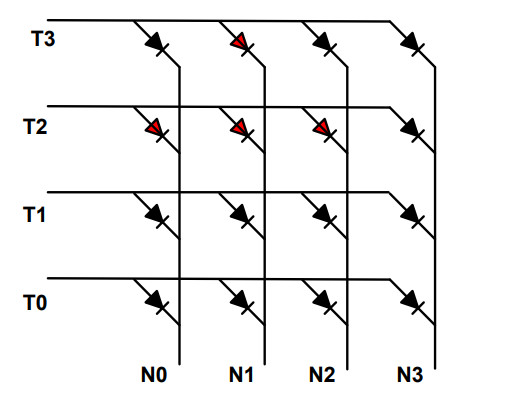
\includegraphics[scale=0.5]{Figures/ledmatrix.jpg} 
	\caption{Matriz de LEDs \protect\footnotemark.}
	\label{fig:matrizled}
\end{figure}

\footnotetext{Imagen tomada de \url{https://web.stanford.edu/class/archive/engr/engr40m.1178/slides_sp17/lecture10.pdf}}

Una de las maneras de habilitar las filas es a través de MOSFET canal P y las columnas se habilitan a través de drivers de LEDs \citep{CONCEPTOMATRIZ}.




\section{ Plataforma de desarrollo DE1SoC}
Para la realización del trabajo se utilizó la plataforma de desarrollo DE1SoC debido a que cumple con los requerimientos y a que la empresa la usó en el desarrollo de proyectos previos. Esto último ahorró mucho tiempo de aprendizaje. Las especificaciones de la plataforma se muestran en la tabla \ref{tab:DE1SOCTABLA}.



La plataforma cuenta con un procesador y un FPGA dentro del mismo \textit{chip} como se puede observar en la figura  \ref{fig:DE1BLOCK}. El FPGA fue usado para controlar la matriz de LEDs debido a su capacidad de manejar varias salidas GPIO en paralelo. Mientras que el procesador fue usado para manejar las comunicaciones.

\begin{table}[h]
\centering
\caption[Especificaciones DE1SoC]{Especificaciones DE1SoC \protect\footnotemark.}
\begin{tabular}{l c c}
\toprule
\textbf{Especificaciones}& \textbf{Detalles}\\
\midrule 


Procesador & ARM CORTEX A9\\
HPS SDRAM & 1 GB DDR3\\
FPGA SDRAM & 64 MB SDRAM\\
UART & UART a USB\\
FLASH & EPCS128\\
Puertos USB & 2\\
Pines GPIO & 36x2\\
Ethernet & 1 Gigabit\\


\bottomrule
\hline
\end{tabular}
\label{tab:DE1SOCTABLA}
\end{table}

\footnotetext{Referencia tomada de \url{https://www.terasic.com.tw/cgi-bin/page/archive.pl?Language=English&CategoryNo=205&No=836&PartNo=1}}


\section{Lenguaje descriptor de hardware}

El lenguaje seleccionado para describir el hardware fue \textit{Verilog} que a pesar de tener una sintaxis muy similar a C difiere en la definición de constantes, requiere la longitud de bits, no tiene estructuras, apuntadores o funciones recursivas. 

En \textit{Verilog} no todas las sentencias del lenguaje son sintetizables. Si las sentencias de todos los módulos son sintetizables, se pueden convertir en una lista de nodos que describe los componentes básicos. ``La lista de nodos puede entonces ser transformada en una forma describiendo las celdas estándar de un circuito integrado, por ejemplo ASIC, o una cadena de bits para un dispositivo de lógica programable (PLD) como puede ser una FPGA o un CPLD'' \citep{WIKIVERILOG}.




\section{Protocolo de comunicaciones UDP}
UDP (Protocolo de Datagrama de Usuario) es un protocolo de comunicaciones que pertenece a la capa de transporte. Permite la transmisión de datos sin conexión preliminar y no define la confirmación de recepción. Se usa en aplicaciones en donde el intercambio de paquetes de la conexión o desconexión son mayores a la información transmitida o en aplicaciones de transmisión de audio y vídeo en tiempo real debido a que retransmitir agregaría retardos \citep{WIKIUDP}.





\pagebreak
\section{Sistema operativo de propósito general para embebidos}

El sistema operativo que se utilizó en el desarrollo de este trabajo fue Linux embebido. Linux embebido se refiere al uso del núcleo en un sistema embebido combinado con un conjunto de utilidades de software libre. 
El núcleo o \textit{kernel} es la interfaz entre el hardware de un PC y sus procesos \citep{KERNEL}. Las tareas que realiza el \textit{kernel} son:

\begin{itemize}
\item Gestión de memoria: control de cantidad de memoria y locación de la misma.
\item Gestión de procesos: administra qué procesos usan la CPU y cuanto tiempo.
\item Controladores de dispositivos: interfaz entre hardware y procesos.
\item Seguridad y llamadas de sistema: recibe solicitud de servicio desde procesos. 
\end{itemize}

\begin{figure}[htpb]
	\centering
	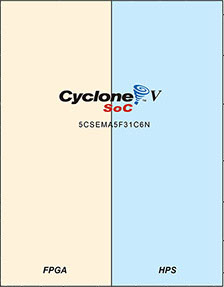
\includegraphics[scale=0.7]{Figures/fpgablock.jpg}  
	\caption{Diagrama de bloques DE1-SoC \protect\footnotemark.}
	\label{fig:DE1BLOCK}
\end{figure}

\footnotetext{Referencia tomada de \url{https://www.terasic.com.tw/attachment/archive/836/image/image_77_thumb.jpg}}


\section{Requerimientos}
En esta sección se indican los requerimientos que fueron propuestos para el proyecto.

\subsection{Grupos de requerimientos asociados con el hardware}

Tarjeta de distribución:
\begin{itemize}
\item Debe tener conectores de entrada IDC40 con la misma distribución de pines usados en las salidas GPIO de la board DE1-SoC.
\item Debe cambiar los niveles de voltaje de 3,3 V a 5 V de todas las entradas. 
\item Debe manejar señales de una frecuencia de entre 5 MHz a 10 MHz.
\item Debe tener conectores de salida IDC16 compatibles con la distribución de pines usados en las matrices de LEDs.
\end{itemize}
Matriz de LEDs:
\begin{itemize}
\item Debe tener un conector de entrada y un conector de salida IDC16.
\item Debe ser capaz de manejar frecuencias de hasta 10 MHz.
\item Debe tener drivers de LEDs con escala de grises de 16 bits.
\item Debe tener 16 LEDs de alto por 16 LEDs de ancho.
\item Debe ser capaz de pasar la información de la entrada a la salida.
\item Debe poder realizarse control por barrido. 
\item La pantalla tendrá una dimensión de 400 píxeles de largo por 96 píxeles de ancho como máximo.
\end{itemize}

\subsection{Grupos de requerimientos asociados con el software}

Sistema operativo:
\begin{itemize}
\item Debe ser capaz de iniciar y restablecer el programa del procesador automáticamente.
\item Debe ser capaz de conectarse a la red LAN. 
\item Debe ser capaz de compartir una carpeta para el proceso de cargado de imágenes.
\item Almacenamiento interno de hasta 500 imágenes.
\end{itemize}

Firmware procesador:
\begin{itemize}
\item Debe ser capaz de leer las imágenes que se encuentran en la carpeta compartida.
\item Debe ser capaz de escribir en una memoria RAM (accesible para el FPGA) las imágenes a ser desplegadas.
\item Debe administrar el despliegue de las imágenes por medio de un archivo externo que sea enviado desde la central de control.
\end{itemize}
\subsection{Grupos de requerimientos asociados al FPGA}
FPGA:
\begin{itemize}
\item El FPGA debe ser capaz de manejar la pantalla LED a una frecuencia de  30 Hz.
\item Debe leer la información de los LEDs de una memoria RAM que comparta con el procesador.
\item Debe manejar los drivers de LEDs a través de una máquina de estado finita.   
\end{itemize}